\documentclass[10pt]{article}
\usepackage[paperwidth=11in,paperheight=8.5in,margin=.4in,footskip=16pt]{geometry}
\usepackage[T1]{fontenc}\usepackage{lmodern}\usepackage{pgfplots}\usepackage{booktabs}
\pgfplotsset{compat=1.18}\definecolor{navy}{RGB}{25,69,102}
\pagestyle{plain}\setlength{\parindent}{0pt}
\begin{document}
\noindent{\Large\bfseries grid / signals-8-offers-12; British; Symmetric risk aversion (alpha=2); cost multiplier 1}\par\smallskip
{\footnotesize Case: \texttt{grid\_\_signals-8-offers-12\_\_complete\_\_ra\_\_cost-1}. Primary profile 1; agreement enabled.}\par\medskip

{\large\bfseries Filing, answering and private exit commitments}\par\smallskip
Filled dots: reached conditional policy. Hollow gray dots: saved off-path policy; the conditional event is undefined.\par
Exit commitments occur privately before the simultaneous agreement decisions.\par\medskip
\begin{tabular}{@{}cc@{}}
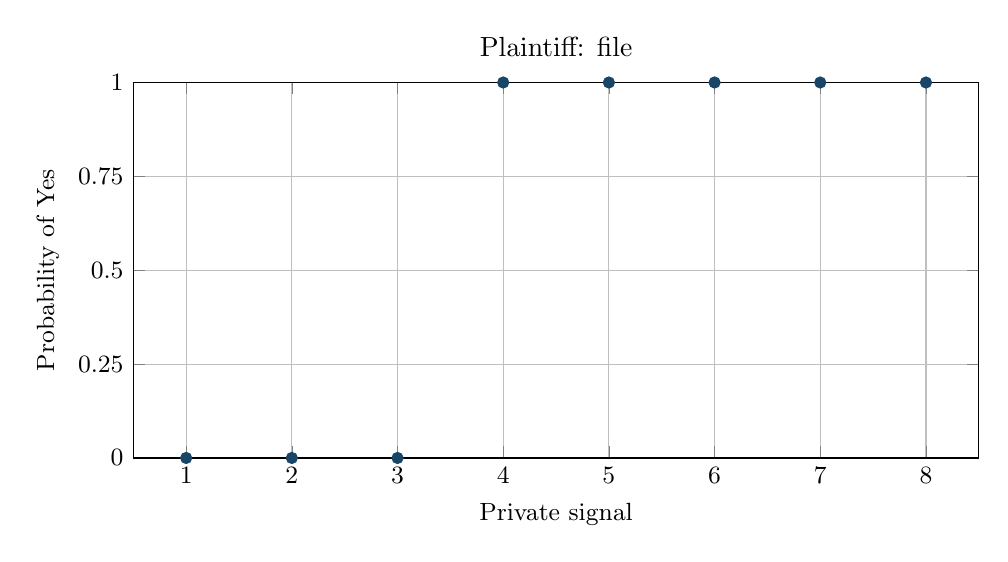
\begin{tikzpicture}\begin{axis}[width=4.85in,height=2.5in,title={Plaintiff: file},xmin=.5,xmax=8.5,ymin=0,ymax=1,xtick={1,...,8},ytick={0,.25,.5,.75,1},xlabel={Private signal},ylabel={Probability of Yes},grid=major,tick label style={font=\small},label style={font=\small},title style={font=\normalsize},clip=false]
\addplot[only marks,mark=*,mark size=2pt,color=navy] coordinates {(1,0) (2,0) (3,0) (4,1) (5,1) (6,1) (7,1) (8,1)};
\addplot[only marks,mark=o,mark size=2.4pt,color=gray] coordinates {};
\end{axis}\end{tikzpicture}&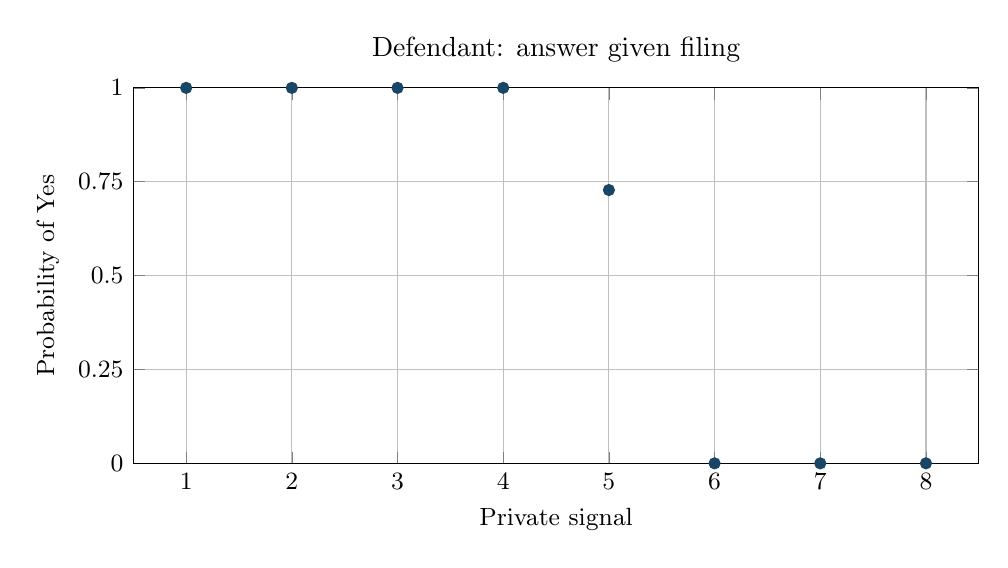
\begin{tikzpicture}\begin{axis}[width=4.85in,height=2.5in,title={Defendant: answer given filing},xmin=.5,xmax=8.5,ymin=0,ymax=1,xtick={1,...,8},ytick={0,.25,.5,.75,1},xlabel={Private signal},ylabel={Probability of Yes},grid=major,tick label style={font=\small},label style={font=\small},title style={font=\normalsize},clip=false]
\addplot[only marks,mark=*,mark size=2pt,color=navy] coordinates {(1,1) (2,1) (3,1) (4,1) (5,0.7279033973767095) (6,0) (7,0) (8,0)};
\addplot[only marks,mark=o,mark size=2.4pt,color=gray] coordinates {};
\end{axis}\end{tikzpicture}\\
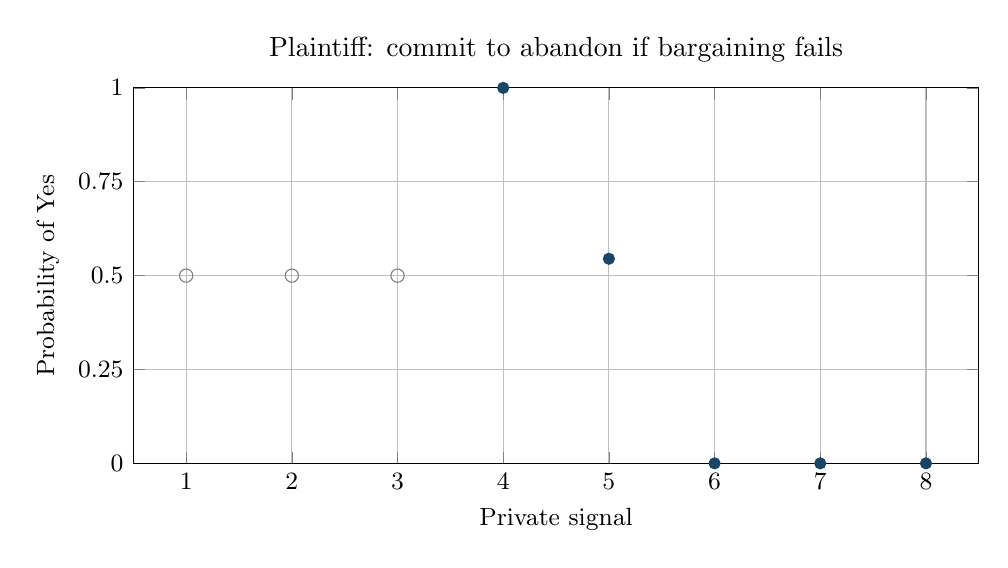
\begin{tikzpicture}\begin{axis}[width=4.85in,height=2.5in,title={Plaintiff: commit to abandon if bargaining fails},xmin=.5,xmax=8.5,ymin=0,ymax=1,xtick={1,...,8},ytick={0,.25,.5,.75,1},xlabel={Private signal},ylabel={Probability of Yes},grid=major,tick label style={font=\small},label style={font=\small},title style={font=\normalsize},clip=false]
\addplot[only marks,mark=*,mark size=2pt,color=navy] coordinates {(4,1) (5,0.54492968251162011) (6,0) (7,0) (8,0)};
\addplot[only marks,mark=o,mark size=2.4pt,color=gray] coordinates {(1,0.5) (2,0.5) (3,0.5)};
\end{axis}\end{tikzpicture}&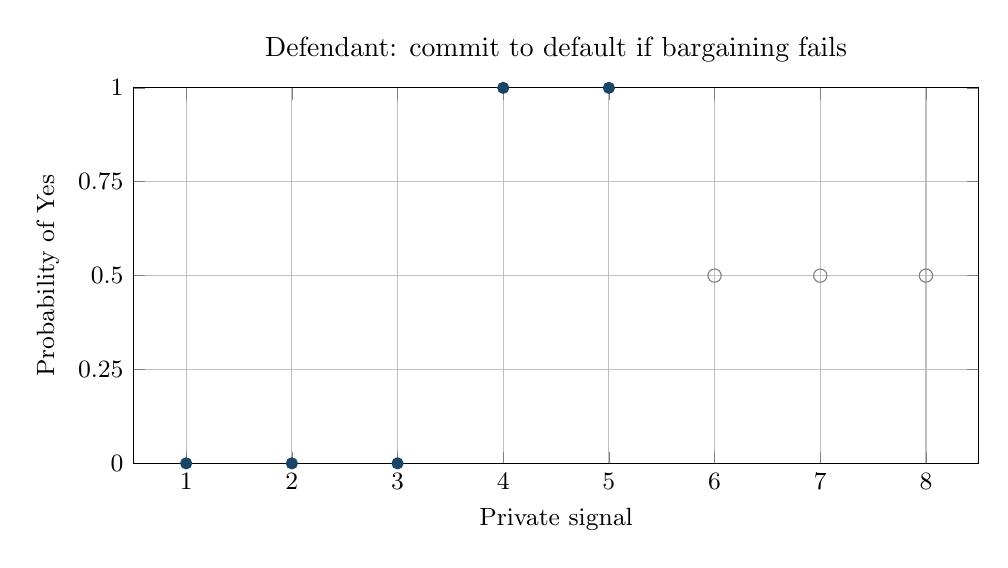
\begin{tikzpicture}\begin{axis}[width=4.85in,height=2.5in,title={Defendant: commit to default if bargaining fails},xmin=.5,xmax=8.5,ymin=0,ymax=1,xtick={1,...,8},ytick={0,.25,.5,.75,1},xlabel={Private signal},ylabel={Probability of Yes},grid=major,tick label style={font=\small},label style={font=\small},title style={font=\normalsize},clip=false]
\addplot[only marks,mark=*,mark size=2pt,color=navy] coordinates {(1,0) (2,0) (3,0) (4,1) (5,1)};
\addplot[only marks,mark=o,mark size=2.4pt,color=gray] coordinates {(6,0.5) (7,0.5) (8,0.5)};
\end{axis}\end{tikzpicture}
\end{tabular}\par\smallskip
{\small Filing: 0.6346; joint filing/answering: 0.2715; answering given filing: 0.4278.}

\newpage
\noindent{\Large\bfseries grid / signals-8-offers-12; British; Symmetric risk aversion (alpha=2); cost multiplier 1}\par\smallskip
{\footnotesize Case: \texttt{grid\_\_signals-8-offers-12\_\_complete\_\_ra\_\_cost-1}. Primary profile 1; agreement enabled.}\par\medskip

{\large\bfseries Agreement conditional on private signal and own exit commitment}\par\smallskip
Both parties choose without observing the other party\textquotesingle s agreement choice or private exit commitment.\par
Offers occur only if both agree. Refusal activates the original commitment-dependent outcomes.\par\medskip
\begin{tabular}{@{}cc@{}}
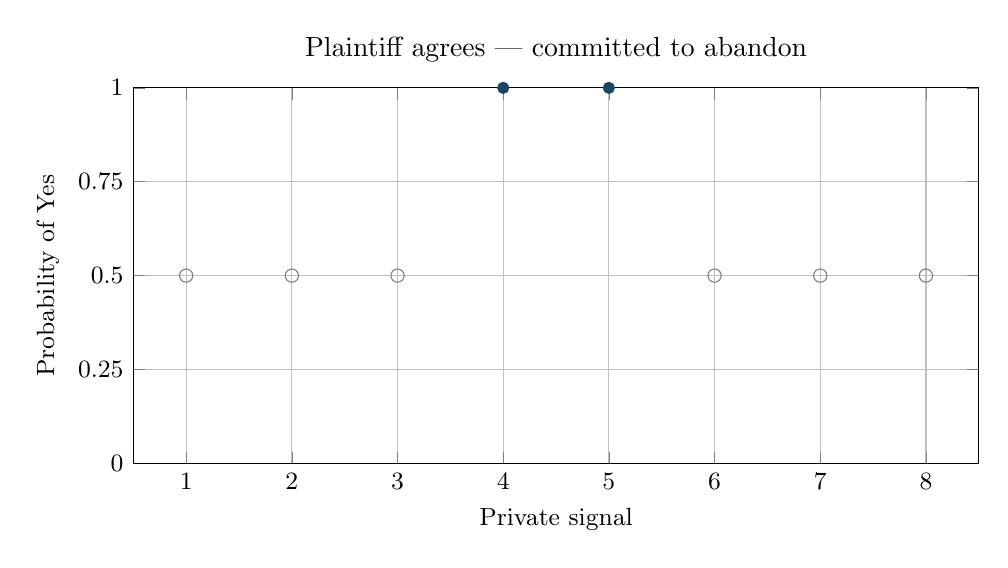
\begin{tikzpicture}\begin{axis}[width=4.85in,height=2.5in,title={Plaintiff agrees | committed to abandon},xmin=.5,xmax=8.5,ymin=0,ymax=1,xtick={1,...,8},ytick={0,.25,.5,.75,1},xlabel={Private signal},ylabel={Probability of Yes},grid=major,tick label style={font=\small},label style={font=\small},title style={font=\normalsize},clip=false]
\addplot[only marks,mark=*,mark size=2pt,color=navy] coordinates {(4,1) (5,1)};
\addplot[only marks,mark=o,mark size=2.4pt,color=gray] coordinates {(1,0.5) (2,0.5) (3,0.5) (6,0.5) (7,0.5) (8,0.5)};
\end{axis}\end{tikzpicture}&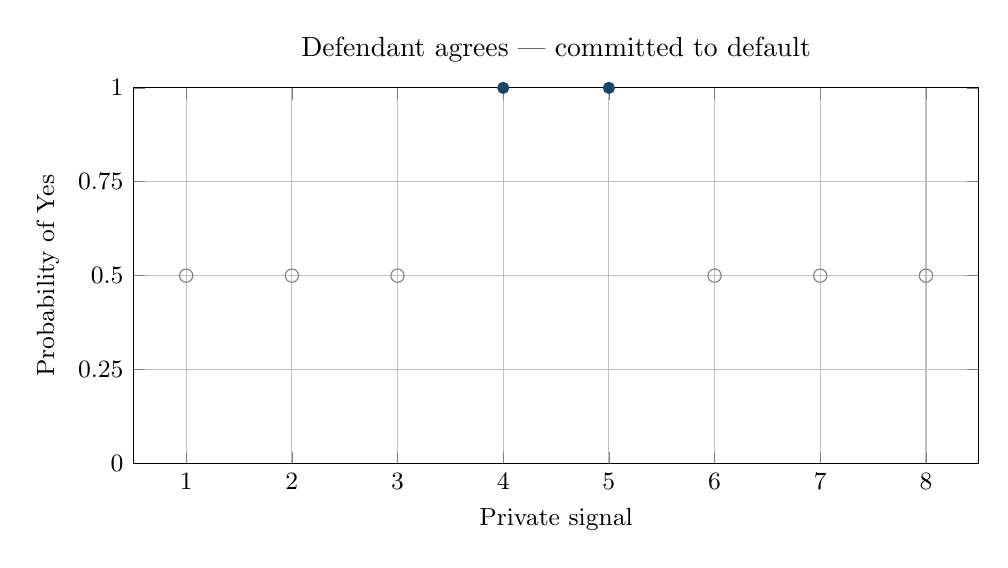
\begin{tikzpicture}\begin{axis}[width=4.85in,height=2.5in,title={Defendant agrees | committed to default},xmin=.5,xmax=8.5,ymin=0,ymax=1,xtick={1,...,8},ytick={0,.25,.5,.75,1},xlabel={Private signal},ylabel={Probability of Yes},grid=major,tick label style={font=\small},label style={font=\small},title style={font=\normalsize},clip=false]
\addplot[only marks,mark=*,mark size=2pt,color=navy] coordinates {(4,1) (5,1)};
\addplot[only marks,mark=o,mark size=2.4pt,color=gray] coordinates {(1,0.5) (2,0.5) (3,0.5) (6,0.5) (7,0.5) (8,0.5)};
\end{axis}\end{tikzpicture}\\
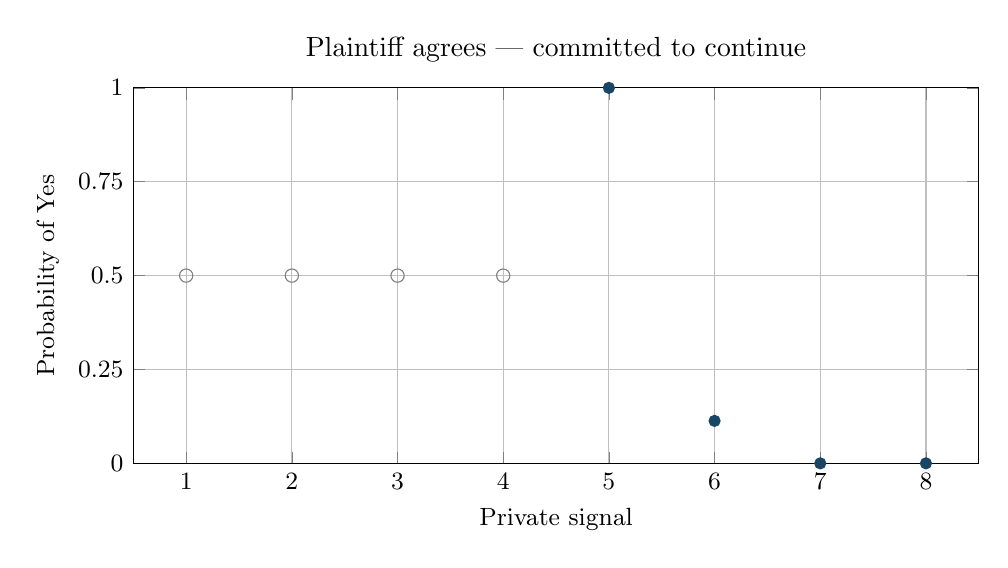
\begin{tikzpicture}\begin{axis}[width=4.85in,height=2.5in,title={Plaintiff agrees | committed to continue},xmin=.5,xmax=8.5,ymin=0,ymax=1,xtick={1,...,8},ytick={0,.25,.5,.75,1},xlabel={Private signal},ylabel={Probability of Yes},grid=major,tick label style={font=\small},label style={font=\small},title style={font=\normalsize},clip=false]
\addplot[only marks,mark=*,mark size=2pt,color=navy] coordinates {(5,1) (6,0.11309053565412421) (7,0) (8,0)};
\addplot[only marks,mark=o,mark size=2.4pt,color=gray] coordinates {(1,0.5) (2,0.5) (3,0.5) (4,0.5)};
\end{axis}\end{tikzpicture}&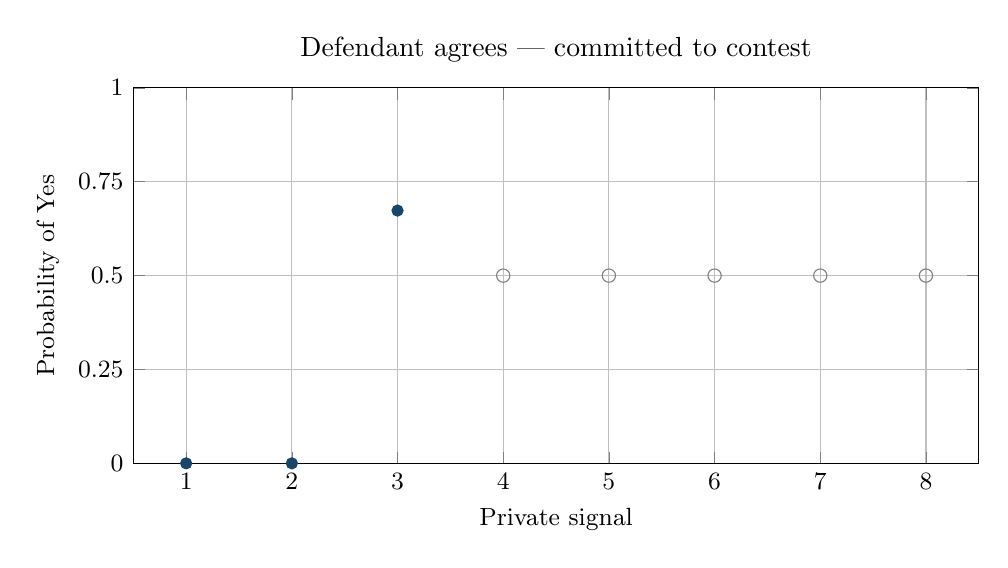
\begin{tikzpicture}\begin{axis}[width=4.85in,height=2.5in,title={Defendant agrees | committed to contest},xmin=.5,xmax=8.5,ymin=0,ymax=1,xtick={1,...,8},ytick={0,.25,.5,.75,1},xlabel={Private signal},ylabel={Probability of Yes},grid=major,tick label style={font=\small},label style={font=\small},title style={font=\normalsize},clip=false]
\addplot[only marks,mark=*,mark size=2pt,color=navy] coordinates {(1,0) (2,0) (3,0.67316396175592041)};
\addplot[only marks,mark=o,mark size=2.4pt,color=gray] coordinates {(4,0.5) (5,0.5) (6,0.5) (7,0.5) (8,0.5)};
\end{axis}\end{tikzpicture}
\end{tabular}\par\smallskip
{\small Joint agreement-stage reach: 0.2715. Conditional joint outcomes: both agree 0.4085; only P declines 0.2989; only D declines 0.2321; both decline 0.06058. These use the full joint signal/history distribution. Hollow dots retain saved off-path policies.}
\newpage
\noindent{\Large\bfseries grid / signals-8-offers-12; British; Symmetric risk aversion (alpha=2); cost multiplier 1}\par\smallskip
{\footnotesize Case: \texttt{grid\_\_signals-8-offers-12\_\_complete\_\_ra\_\_cost-1}. Primary profile 1; agreement enabled.}\par\medskip

{\large\bfseries Complete mixed offer distributions}\par\smallskip
Rows show the saved policy at each private signal and own commitment, after both parties agree to bargain.\par
An asterisk marks an unreachable information set: its saved completion is shown, but no reached conditional distribution exists.\par\medskip
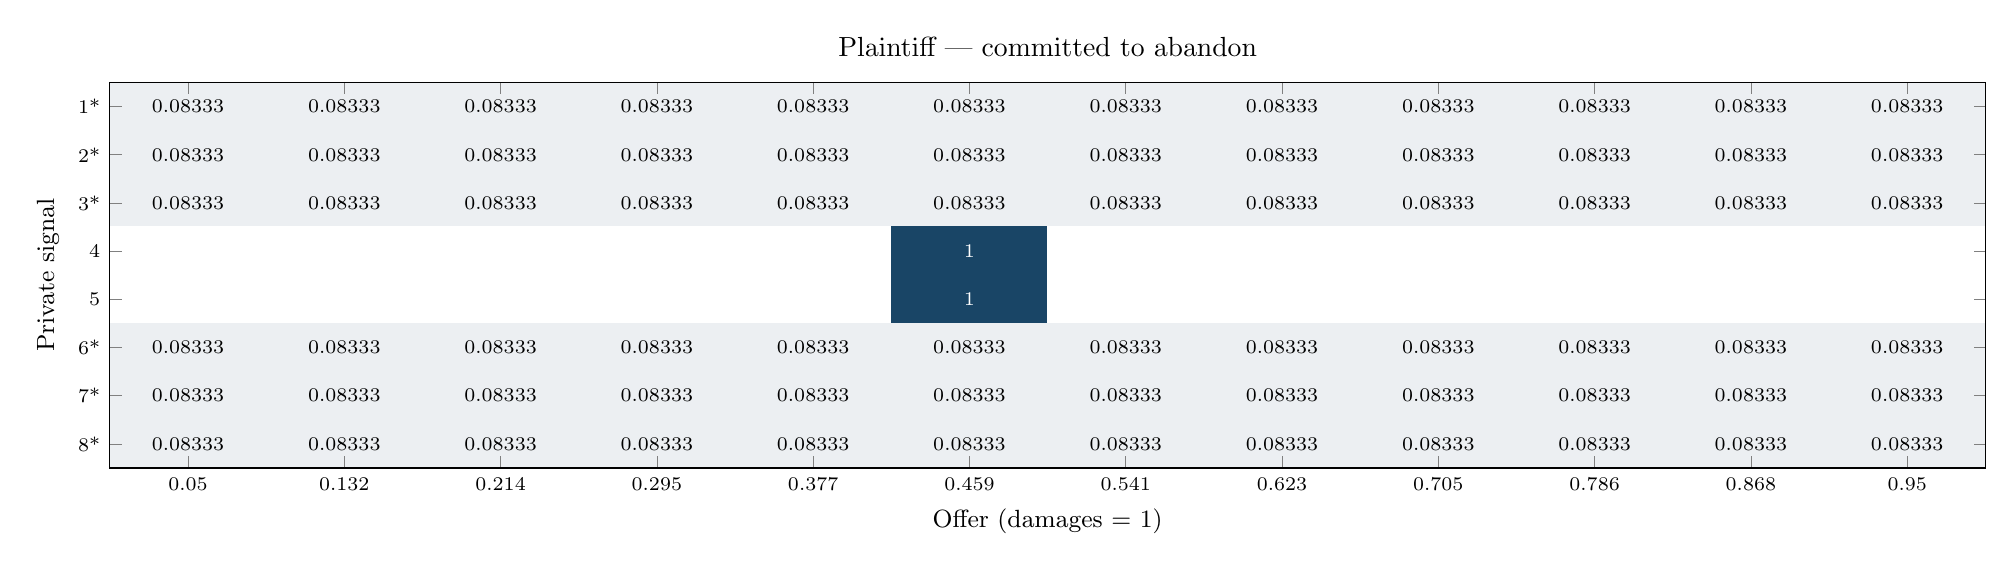
\begin{tikzpicture}\begin{axis}[
width=10.0in,height=2.55in,title={Plaintiff | committed to abandon},
xmin=.5,xmax=12.5,ymin=.5,ymax=8.5,y dir=reverse,
xtick={1,...,12},xticklabels={0.05,0.132,0.214,0.295,0.377,0.459,0.541,0.623,0.705,0.786,0.868,0.95},
ytick={1,...,8},yticklabels={1*,2*,3*,4,5,6*,7*,8*},
xlabel={Offer (damages = 1)},ylabel={Private signal},
tick label style={font=\scriptsize},label style={font=\small},title style={font=\normalsize},
colormap={policy}{color(0cm)=(white);color(1cm)=(navy)},point meta min=0,point meta max=1,axis on top,clip=false]
\addplot[matrix plot*,mesh/cols=12,point meta=explicit] table[meta=p] {
x y p
1 1 0.083333333333333343
2 1 0.083333333333333343
3 1 0.083333333333333343
4 1 0.083333333333333343
5 1 0.083333333333333343
6 1 0.083333333333333343
7 1 0.083333333333333343
8 1 0.083333333333333343
9 1 0.083333333333333343
10 1 0.083333333333333343
11 1 0.083333333333333343
12 1 0.083333333333333343
1 2 0.083333333333333343
2 2 0.083333333333333343
3 2 0.083333333333333343
4 2 0.083333333333333343
5 2 0.083333333333333343
6 2 0.083333333333333343
7 2 0.083333333333333343
8 2 0.083333333333333343
9 2 0.083333333333333343
10 2 0.083333333333333343
11 2 0.083333333333333343
12 2 0.083333333333333343
1 3 0.083333333333333343
2 3 0.083333333333333343
3 3 0.083333333333333343
4 3 0.083333333333333343
5 3 0.083333333333333343
6 3 0.083333333333333343
7 3 0.083333333333333343
8 3 0.083333333333333343
9 3 0.083333333333333343
10 3 0.083333333333333343
11 3 0.083333333333333343
12 3 0.083333333333333343
1 4 0
2 4 0
3 4 0
4 4 0
5 4 0
6 4 1
7 4 0
8 4 0
9 4 0
10 4 0
11 4 0
12 4 0
1 5 0
2 5 0
3 5 0
4 5 0
5 5 0
6 5 1
7 5 0
8 5 0
9 5 0
10 5 0
11 5 0
12 5 0
1 6 0.083333333333333343
2 6 0.083333333333333343
3 6 0.083333333333333343
4 6 0.083333333333333343
5 6 0.083333333333333343
6 6 0.083333333333333343
7 6 0.083333333333333343
8 6 0.083333333333333343
9 6 0.083333333333333343
10 6 0.083333333333333343
11 6 0.083333333333333343
12 6 0.083333333333333343
1 7 0.083333333333333343
2 7 0.083333333333333343
3 7 0.083333333333333343
4 7 0.083333333333333343
5 7 0.083333333333333343
6 7 0.083333333333333343
7 7 0.083333333333333343
8 7 0.083333333333333343
9 7 0.083333333333333343
10 7 0.083333333333333343
11 7 0.083333333333333343
12 7 0.083333333333333343
1 8 0.083333333333333343
2 8 0.083333333333333343
3 8 0.083333333333333343
4 8 0.083333333333333343
5 8 0.083333333333333343
6 8 0.083333333333333343
7 8 0.083333333333333343
8 8 0.083333333333333343
9 8 0.083333333333333343
10 8 0.083333333333333343
11 8 0.083333333333333343
12 8 0.083333333333333343
};
\node[font=\scriptsize,text=black] at (axis cs:1,1) {0.08333};
\node[font=\scriptsize,text=black] at (axis cs:2,1) {0.08333};
\node[font=\scriptsize,text=black] at (axis cs:3,1) {0.08333};
\node[font=\scriptsize,text=black] at (axis cs:4,1) {0.08333};
\node[font=\scriptsize,text=black] at (axis cs:5,1) {0.08333};
\node[font=\scriptsize,text=black] at (axis cs:6,1) {0.08333};
\node[font=\scriptsize,text=black] at (axis cs:7,1) {0.08333};
\node[font=\scriptsize,text=black] at (axis cs:8,1) {0.08333};
\node[font=\scriptsize,text=black] at (axis cs:9,1) {0.08333};
\node[font=\scriptsize,text=black] at (axis cs:10,1) {0.08333};
\node[font=\scriptsize,text=black] at (axis cs:11,1) {0.08333};
\node[font=\scriptsize,text=black] at (axis cs:12,1) {0.08333};
\node[font=\scriptsize,text=black] at (axis cs:1,2) {0.08333};
\node[font=\scriptsize,text=black] at (axis cs:2,2) {0.08333};
\node[font=\scriptsize,text=black] at (axis cs:3,2) {0.08333};
\node[font=\scriptsize,text=black] at (axis cs:4,2) {0.08333};
\node[font=\scriptsize,text=black] at (axis cs:5,2) {0.08333};
\node[font=\scriptsize,text=black] at (axis cs:6,2) {0.08333};
\node[font=\scriptsize,text=black] at (axis cs:7,2) {0.08333};
\node[font=\scriptsize,text=black] at (axis cs:8,2) {0.08333};
\node[font=\scriptsize,text=black] at (axis cs:9,2) {0.08333};
\node[font=\scriptsize,text=black] at (axis cs:10,2) {0.08333};
\node[font=\scriptsize,text=black] at (axis cs:11,2) {0.08333};
\node[font=\scriptsize,text=black] at (axis cs:12,2) {0.08333};
\node[font=\scriptsize,text=black] at (axis cs:1,3) {0.08333};
\node[font=\scriptsize,text=black] at (axis cs:2,3) {0.08333};
\node[font=\scriptsize,text=black] at (axis cs:3,3) {0.08333};
\node[font=\scriptsize,text=black] at (axis cs:4,3) {0.08333};
\node[font=\scriptsize,text=black] at (axis cs:5,3) {0.08333};
\node[font=\scriptsize,text=black] at (axis cs:6,3) {0.08333};
\node[font=\scriptsize,text=black] at (axis cs:7,3) {0.08333};
\node[font=\scriptsize,text=black] at (axis cs:8,3) {0.08333};
\node[font=\scriptsize,text=black] at (axis cs:9,3) {0.08333};
\node[font=\scriptsize,text=black] at (axis cs:10,3) {0.08333};
\node[font=\scriptsize,text=black] at (axis cs:11,3) {0.08333};
\node[font=\scriptsize,text=black] at (axis cs:12,3) {0.08333};
\node[font=\scriptsize,text=white] at (axis cs:6,4) {1};
\node[font=\scriptsize,text=white] at (axis cs:6,5) {1};
\node[font=\scriptsize,text=black] at (axis cs:1,6) {0.08333};
\node[font=\scriptsize,text=black] at (axis cs:2,6) {0.08333};
\node[font=\scriptsize,text=black] at (axis cs:3,6) {0.08333};
\node[font=\scriptsize,text=black] at (axis cs:4,6) {0.08333};
\node[font=\scriptsize,text=black] at (axis cs:5,6) {0.08333};
\node[font=\scriptsize,text=black] at (axis cs:6,6) {0.08333};
\node[font=\scriptsize,text=black] at (axis cs:7,6) {0.08333};
\node[font=\scriptsize,text=black] at (axis cs:8,6) {0.08333};
\node[font=\scriptsize,text=black] at (axis cs:9,6) {0.08333};
\node[font=\scriptsize,text=black] at (axis cs:10,6) {0.08333};
\node[font=\scriptsize,text=black] at (axis cs:11,6) {0.08333};
\node[font=\scriptsize,text=black] at (axis cs:12,6) {0.08333};
\node[font=\scriptsize,text=black] at (axis cs:1,7) {0.08333};
\node[font=\scriptsize,text=black] at (axis cs:2,7) {0.08333};
\node[font=\scriptsize,text=black] at (axis cs:3,7) {0.08333};
\node[font=\scriptsize,text=black] at (axis cs:4,7) {0.08333};
\node[font=\scriptsize,text=black] at (axis cs:5,7) {0.08333};
\node[font=\scriptsize,text=black] at (axis cs:6,7) {0.08333};
\node[font=\scriptsize,text=black] at (axis cs:7,7) {0.08333};
\node[font=\scriptsize,text=black] at (axis cs:8,7) {0.08333};
\node[font=\scriptsize,text=black] at (axis cs:9,7) {0.08333};
\node[font=\scriptsize,text=black] at (axis cs:10,7) {0.08333};
\node[font=\scriptsize,text=black] at (axis cs:11,7) {0.08333};
\node[font=\scriptsize,text=black] at (axis cs:12,7) {0.08333};
\node[font=\scriptsize,text=black] at (axis cs:1,8) {0.08333};
\node[font=\scriptsize,text=black] at (axis cs:2,8) {0.08333};
\node[font=\scriptsize,text=black] at (axis cs:3,8) {0.08333};
\node[font=\scriptsize,text=black] at (axis cs:4,8) {0.08333};
\node[font=\scriptsize,text=black] at (axis cs:5,8) {0.08333};
\node[font=\scriptsize,text=black] at (axis cs:6,8) {0.08333};
\node[font=\scriptsize,text=black] at (axis cs:7,8) {0.08333};
\node[font=\scriptsize,text=black] at (axis cs:8,8) {0.08333};
\node[font=\scriptsize,text=black] at (axis cs:9,8) {0.08333};
\node[font=\scriptsize,text=black] at (axis cs:10,8) {0.08333};
\node[font=\scriptsize,text=black] at (axis cs:11,8) {0.08333};
\node[font=\scriptsize,text=black] at (axis cs:12,8) {0.08333};
\end{axis}\end{tikzpicture}
\par\medskip
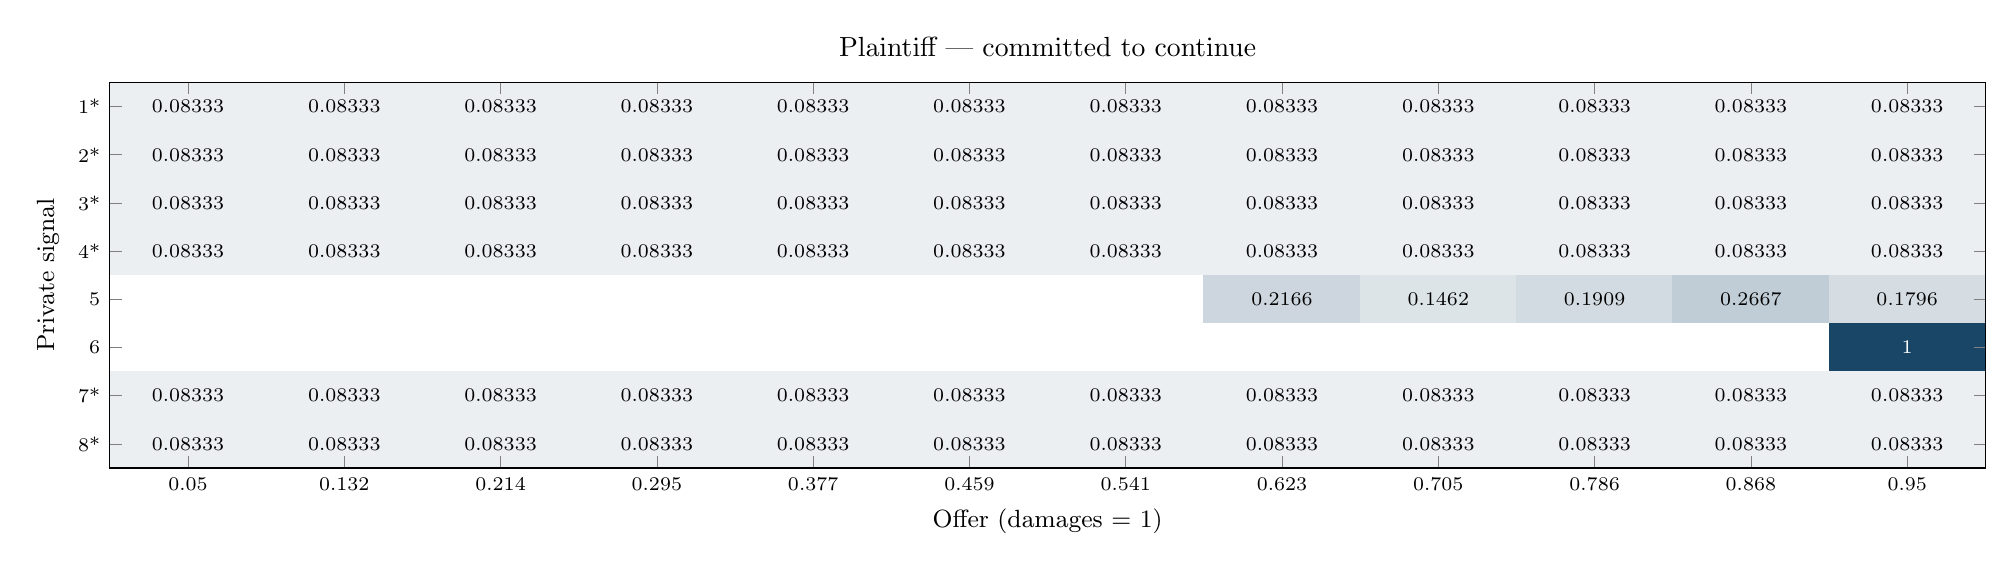
\begin{tikzpicture}\begin{axis}[
width=10.0in,height=2.55in,title={Plaintiff | committed to continue},
xmin=.5,xmax=12.5,ymin=.5,ymax=8.5,y dir=reverse,
xtick={1,...,12},xticklabels={0.05,0.132,0.214,0.295,0.377,0.459,0.541,0.623,0.705,0.786,0.868,0.95},
ytick={1,...,8},yticklabels={1*,2*,3*,4*,5,6,7*,8*},
xlabel={Offer (damages = 1)},ylabel={Private signal},
tick label style={font=\scriptsize},label style={font=\small},title style={font=\normalsize},
colormap={policy}{color(0cm)=(white);color(1cm)=(navy)},point meta min=0,point meta max=1,axis on top,clip=false]
\addplot[matrix plot*,mesh/cols=12,point meta=explicit] table[meta=p] {
x y p
1 1 0.083333333333333343
2 1 0.083333333333333343
3 1 0.083333333333333343
4 1 0.083333333333333343
5 1 0.083333333333333343
6 1 0.083333333333333343
7 1 0.083333333333333343
8 1 0.083333333333333343
9 1 0.083333333333333343
10 1 0.083333333333333343
11 1 0.083333333333333343
12 1 0.083333333333333343
1 2 0.083333333333333343
2 2 0.083333333333333343
3 2 0.083333333333333343
4 2 0.083333333333333343
5 2 0.083333333333333343
6 2 0.083333333333333343
7 2 0.083333333333333343
8 2 0.083333333333333343
9 2 0.083333333333333343
10 2 0.083333333333333343
11 2 0.083333333333333343
12 2 0.083333333333333343
1 3 0.083333333333333343
2 3 0.083333333333333343
3 3 0.083333333333333343
4 3 0.083333333333333343
5 3 0.083333333333333343
6 3 0.083333333333333343
7 3 0.083333333333333343
8 3 0.083333333333333343
9 3 0.083333333333333343
10 3 0.083333333333333343
11 3 0.083333333333333343
12 3 0.083333333333333343
1 4 0.083333333333333343
2 4 0.083333333333333343
3 4 0.083333333333333343
4 4 0.083333333333333343
5 4 0.083333333333333343
6 4 0.083333333333333343
7 4 0.083333333333333343
8 4 0.083333333333333343
9 4 0.083333333333333343
10 4 0.083333333333333343
11 4 0.083333333333333343
12 4 0.083333333333333343
1 5 0
2 5 0
3 5 0
4 5 0
5 5 0
6 5 0
7 5 0
8 5 0.21662475385048569
9 5 0.14616305681562233
10 5 0.19088744939734043
11 5 0.2666867453112311
12 5 0.17963799462532051
1 6 0
2 6 0
3 6 0
4 6 0
5 6 0
6 6 0
7 6 0
8 6 0
9 6 0
10 6 0
11 6 0
12 6 1
1 7 0.083333333333333343
2 7 0.083333333333333343
3 7 0.083333333333333343
4 7 0.083333333333333343
5 7 0.083333333333333343
6 7 0.083333333333333343
7 7 0.083333333333333343
8 7 0.083333333333333343
9 7 0.083333333333333343
10 7 0.083333333333333343
11 7 0.083333333333333343
12 7 0.083333333333333343
1 8 0.083333333333333343
2 8 0.083333333333333343
3 8 0.083333333333333343
4 8 0.083333333333333343
5 8 0.083333333333333343
6 8 0.083333333333333343
7 8 0.083333333333333343
8 8 0.083333333333333343
9 8 0.083333333333333343
10 8 0.083333333333333343
11 8 0.083333333333333343
12 8 0.083333333333333343
};
\node[font=\scriptsize,text=black] at (axis cs:1,1) {0.08333};
\node[font=\scriptsize,text=black] at (axis cs:2,1) {0.08333};
\node[font=\scriptsize,text=black] at (axis cs:3,1) {0.08333};
\node[font=\scriptsize,text=black] at (axis cs:4,1) {0.08333};
\node[font=\scriptsize,text=black] at (axis cs:5,1) {0.08333};
\node[font=\scriptsize,text=black] at (axis cs:6,1) {0.08333};
\node[font=\scriptsize,text=black] at (axis cs:7,1) {0.08333};
\node[font=\scriptsize,text=black] at (axis cs:8,1) {0.08333};
\node[font=\scriptsize,text=black] at (axis cs:9,1) {0.08333};
\node[font=\scriptsize,text=black] at (axis cs:10,1) {0.08333};
\node[font=\scriptsize,text=black] at (axis cs:11,1) {0.08333};
\node[font=\scriptsize,text=black] at (axis cs:12,1) {0.08333};
\node[font=\scriptsize,text=black] at (axis cs:1,2) {0.08333};
\node[font=\scriptsize,text=black] at (axis cs:2,2) {0.08333};
\node[font=\scriptsize,text=black] at (axis cs:3,2) {0.08333};
\node[font=\scriptsize,text=black] at (axis cs:4,2) {0.08333};
\node[font=\scriptsize,text=black] at (axis cs:5,2) {0.08333};
\node[font=\scriptsize,text=black] at (axis cs:6,2) {0.08333};
\node[font=\scriptsize,text=black] at (axis cs:7,2) {0.08333};
\node[font=\scriptsize,text=black] at (axis cs:8,2) {0.08333};
\node[font=\scriptsize,text=black] at (axis cs:9,2) {0.08333};
\node[font=\scriptsize,text=black] at (axis cs:10,2) {0.08333};
\node[font=\scriptsize,text=black] at (axis cs:11,2) {0.08333};
\node[font=\scriptsize,text=black] at (axis cs:12,2) {0.08333};
\node[font=\scriptsize,text=black] at (axis cs:1,3) {0.08333};
\node[font=\scriptsize,text=black] at (axis cs:2,3) {0.08333};
\node[font=\scriptsize,text=black] at (axis cs:3,3) {0.08333};
\node[font=\scriptsize,text=black] at (axis cs:4,3) {0.08333};
\node[font=\scriptsize,text=black] at (axis cs:5,3) {0.08333};
\node[font=\scriptsize,text=black] at (axis cs:6,3) {0.08333};
\node[font=\scriptsize,text=black] at (axis cs:7,3) {0.08333};
\node[font=\scriptsize,text=black] at (axis cs:8,3) {0.08333};
\node[font=\scriptsize,text=black] at (axis cs:9,3) {0.08333};
\node[font=\scriptsize,text=black] at (axis cs:10,3) {0.08333};
\node[font=\scriptsize,text=black] at (axis cs:11,3) {0.08333};
\node[font=\scriptsize,text=black] at (axis cs:12,3) {0.08333};
\node[font=\scriptsize,text=black] at (axis cs:1,4) {0.08333};
\node[font=\scriptsize,text=black] at (axis cs:2,4) {0.08333};
\node[font=\scriptsize,text=black] at (axis cs:3,4) {0.08333};
\node[font=\scriptsize,text=black] at (axis cs:4,4) {0.08333};
\node[font=\scriptsize,text=black] at (axis cs:5,4) {0.08333};
\node[font=\scriptsize,text=black] at (axis cs:6,4) {0.08333};
\node[font=\scriptsize,text=black] at (axis cs:7,4) {0.08333};
\node[font=\scriptsize,text=black] at (axis cs:8,4) {0.08333};
\node[font=\scriptsize,text=black] at (axis cs:9,4) {0.08333};
\node[font=\scriptsize,text=black] at (axis cs:10,4) {0.08333};
\node[font=\scriptsize,text=black] at (axis cs:11,4) {0.08333};
\node[font=\scriptsize,text=black] at (axis cs:12,4) {0.08333};
\node[font=\scriptsize,text=black] at (axis cs:8,5) {0.2166};
\node[font=\scriptsize,text=black] at (axis cs:9,5) {0.1462};
\node[font=\scriptsize,text=black] at (axis cs:10,5) {0.1909};
\node[font=\scriptsize,text=black] at (axis cs:11,5) {0.2667};
\node[font=\scriptsize,text=black] at (axis cs:12,5) {0.1796};
\node[font=\scriptsize,text=white] at (axis cs:12,6) {1};
\node[font=\scriptsize,text=black] at (axis cs:1,7) {0.08333};
\node[font=\scriptsize,text=black] at (axis cs:2,7) {0.08333};
\node[font=\scriptsize,text=black] at (axis cs:3,7) {0.08333};
\node[font=\scriptsize,text=black] at (axis cs:4,7) {0.08333};
\node[font=\scriptsize,text=black] at (axis cs:5,7) {0.08333};
\node[font=\scriptsize,text=black] at (axis cs:6,7) {0.08333};
\node[font=\scriptsize,text=black] at (axis cs:7,7) {0.08333};
\node[font=\scriptsize,text=black] at (axis cs:8,7) {0.08333};
\node[font=\scriptsize,text=black] at (axis cs:9,7) {0.08333};
\node[font=\scriptsize,text=black] at (axis cs:10,7) {0.08333};
\node[font=\scriptsize,text=black] at (axis cs:11,7) {0.08333};
\node[font=\scriptsize,text=black] at (axis cs:12,7) {0.08333};
\node[font=\scriptsize,text=black] at (axis cs:1,8) {0.08333};
\node[font=\scriptsize,text=black] at (axis cs:2,8) {0.08333};
\node[font=\scriptsize,text=black] at (axis cs:3,8) {0.08333};
\node[font=\scriptsize,text=black] at (axis cs:4,8) {0.08333};
\node[font=\scriptsize,text=black] at (axis cs:5,8) {0.08333};
\node[font=\scriptsize,text=black] at (axis cs:6,8) {0.08333};
\node[font=\scriptsize,text=black] at (axis cs:7,8) {0.08333};
\node[font=\scriptsize,text=black] at (axis cs:8,8) {0.08333};
\node[font=\scriptsize,text=black] at (axis cs:9,8) {0.08333};
\node[font=\scriptsize,text=black] at (axis cs:10,8) {0.08333};
\node[font=\scriptsize,text=black] at (axis cs:11,8) {0.08333};
\node[font=\scriptsize,text=black] at (axis cs:12,8) {0.08333};
\end{axis}\end{tikzpicture}
\par\smallskip
{\small Color and cell labels show action probabilities (white = 0; darkest blue = 1). Empty cell labels mean exact zero.
Every positive entry is printed, including arbitrarily small probabilities. Full precision is retained in the editable TeX and profile JSON.}
\newpage
\noindent{\Large\bfseries grid / signals-8-offers-12; British; Symmetric risk aversion (alpha=2); cost multiplier 1}\par\smallskip
{\footnotesize Case: \texttt{grid\_\_signals-8-offers-12\_\_complete\_\_ra\_\_cost-1}. Primary profile 1; agreement enabled.}\par\medskip

{\large\bfseries Complete mixed offer distributions}\par\smallskip
Rows show the saved policy at each private signal and own commitment, after both parties agree to bargain.\par
An asterisk marks an unreachable information set: its saved completion is shown, but no reached conditional distribution exists.\par\medskip
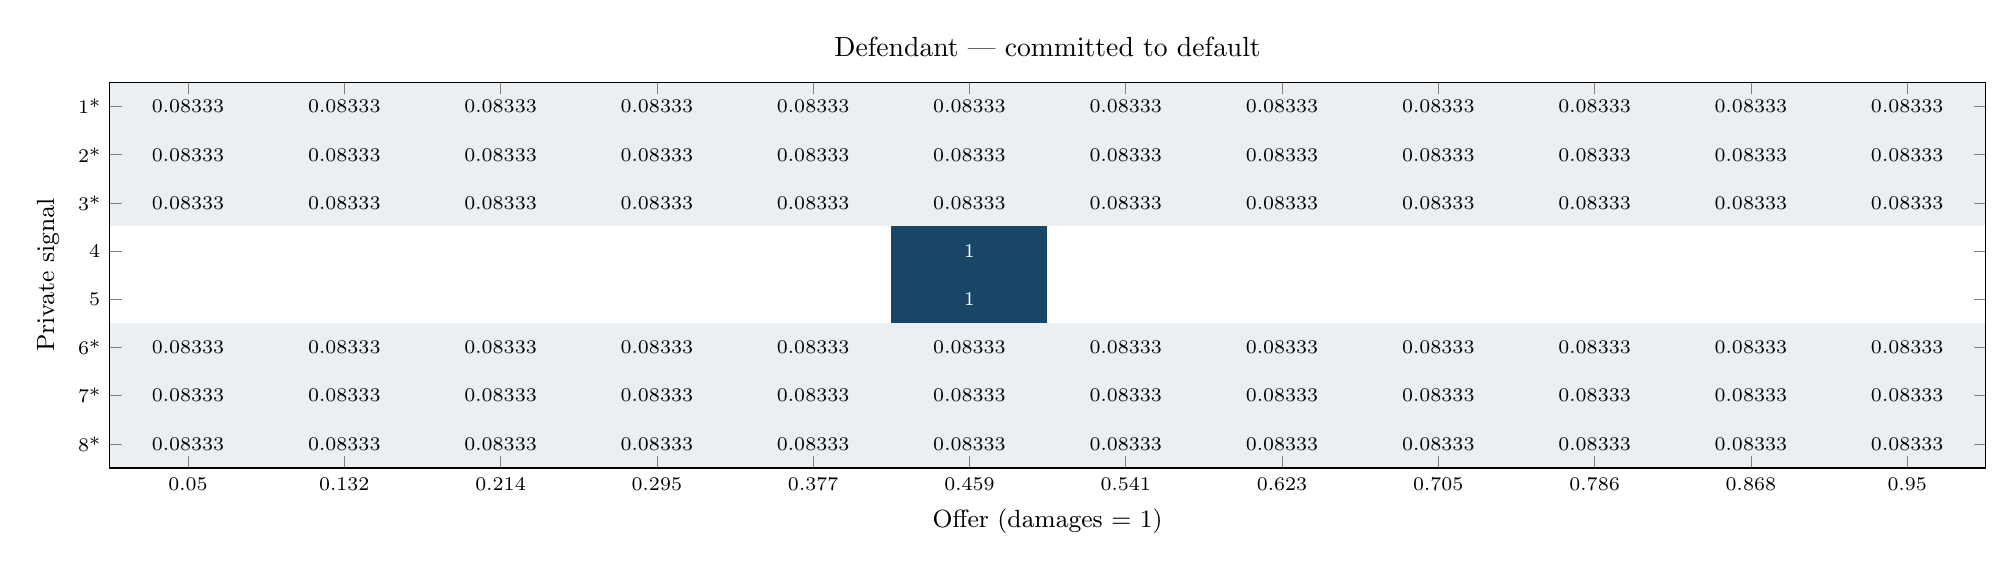
\begin{tikzpicture}\begin{axis}[
width=10.0in,height=2.55in,title={Defendant | committed to default},
xmin=.5,xmax=12.5,ymin=.5,ymax=8.5,y dir=reverse,
xtick={1,...,12},xticklabels={0.05,0.132,0.214,0.295,0.377,0.459,0.541,0.623,0.705,0.786,0.868,0.95},
ytick={1,...,8},yticklabels={1*,2*,3*,4,5,6*,7*,8*},
xlabel={Offer (damages = 1)},ylabel={Private signal},
tick label style={font=\scriptsize},label style={font=\small},title style={font=\normalsize},
colormap={policy}{color(0cm)=(white);color(1cm)=(navy)},point meta min=0,point meta max=1,axis on top,clip=false]
\addplot[matrix plot*,mesh/cols=12,point meta=explicit] table[meta=p] {
x y p
1 1 0.083333333333333343
2 1 0.083333333333333343
3 1 0.083333333333333343
4 1 0.083333333333333343
5 1 0.083333333333333343
6 1 0.083333333333333343
7 1 0.083333333333333343
8 1 0.083333333333333343
9 1 0.083333333333333343
10 1 0.083333333333333343
11 1 0.083333333333333343
12 1 0.083333333333333343
1 2 0.083333333333333343
2 2 0.083333333333333343
3 2 0.083333333333333343
4 2 0.083333333333333343
5 2 0.083333333333333343
6 2 0.083333333333333343
7 2 0.083333333333333343
8 2 0.083333333333333343
9 2 0.083333333333333343
10 2 0.083333333333333343
11 2 0.083333333333333343
12 2 0.083333333333333343
1 3 0.083333333333333343
2 3 0.083333333333333343
3 3 0.083333333333333343
4 3 0.083333333333333343
5 3 0.083333333333333343
6 3 0.083333333333333343
7 3 0.083333333333333343
8 3 0.083333333333333343
9 3 0.083333333333333343
10 3 0.083333333333333343
11 3 0.083333333333333343
12 3 0.083333333333333343
1 4 0
2 4 0
3 4 0
4 4 0
5 4 0
6 4 1
7 4 0
8 4 0
9 4 0
10 4 0
11 4 0
12 4 0
1 5 0
2 5 0
3 5 0
4 5 0
5 5 0
6 5 1
7 5 0
8 5 0
9 5 0
10 5 0
11 5 0
12 5 0
1 6 0.083333333333333343
2 6 0.083333333333333343
3 6 0.083333333333333343
4 6 0.083333333333333343
5 6 0.083333333333333343
6 6 0.083333333333333343
7 6 0.083333333333333343
8 6 0.083333333333333343
9 6 0.083333333333333343
10 6 0.083333333333333343
11 6 0.083333333333333343
12 6 0.083333333333333343
1 7 0.083333333333333343
2 7 0.083333333333333343
3 7 0.083333333333333343
4 7 0.083333333333333343
5 7 0.083333333333333343
6 7 0.083333333333333343
7 7 0.083333333333333343
8 7 0.083333333333333343
9 7 0.083333333333333343
10 7 0.083333333333333343
11 7 0.083333333333333343
12 7 0.083333333333333343
1 8 0.083333333333333343
2 8 0.083333333333333343
3 8 0.083333333333333343
4 8 0.083333333333333343
5 8 0.083333333333333343
6 8 0.083333333333333343
7 8 0.083333333333333343
8 8 0.083333333333333343
9 8 0.083333333333333343
10 8 0.083333333333333343
11 8 0.083333333333333343
12 8 0.083333333333333343
};
\node[font=\scriptsize,text=black] at (axis cs:1,1) {0.08333};
\node[font=\scriptsize,text=black] at (axis cs:2,1) {0.08333};
\node[font=\scriptsize,text=black] at (axis cs:3,1) {0.08333};
\node[font=\scriptsize,text=black] at (axis cs:4,1) {0.08333};
\node[font=\scriptsize,text=black] at (axis cs:5,1) {0.08333};
\node[font=\scriptsize,text=black] at (axis cs:6,1) {0.08333};
\node[font=\scriptsize,text=black] at (axis cs:7,1) {0.08333};
\node[font=\scriptsize,text=black] at (axis cs:8,1) {0.08333};
\node[font=\scriptsize,text=black] at (axis cs:9,1) {0.08333};
\node[font=\scriptsize,text=black] at (axis cs:10,1) {0.08333};
\node[font=\scriptsize,text=black] at (axis cs:11,1) {0.08333};
\node[font=\scriptsize,text=black] at (axis cs:12,1) {0.08333};
\node[font=\scriptsize,text=black] at (axis cs:1,2) {0.08333};
\node[font=\scriptsize,text=black] at (axis cs:2,2) {0.08333};
\node[font=\scriptsize,text=black] at (axis cs:3,2) {0.08333};
\node[font=\scriptsize,text=black] at (axis cs:4,2) {0.08333};
\node[font=\scriptsize,text=black] at (axis cs:5,2) {0.08333};
\node[font=\scriptsize,text=black] at (axis cs:6,2) {0.08333};
\node[font=\scriptsize,text=black] at (axis cs:7,2) {0.08333};
\node[font=\scriptsize,text=black] at (axis cs:8,2) {0.08333};
\node[font=\scriptsize,text=black] at (axis cs:9,2) {0.08333};
\node[font=\scriptsize,text=black] at (axis cs:10,2) {0.08333};
\node[font=\scriptsize,text=black] at (axis cs:11,2) {0.08333};
\node[font=\scriptsize,text=black] at (axis cs:12,2) {0.08333};
\node[font=\scriptsize,text=black] at (axis cs:1,3) {0.08333};
\node[font=\scriptsize,text=black] at (axis cs:2,3) {0.08333};
\node[font=\scriptsize,text=black] at (axis cs:3,3) {0.08333};
\node[font=\scriptsize,text=black] at (axis cs:4,3) {0.08333};
\node[font=\scriptsize,text=black] at (axis cs:5,3) {0.08333};
\node[font=\scriptsize,text=black] at (axis cs:6,3) {0.08333};
\node[font=\scriptsize,text=black] at (axis cs:7,3) {0.08333};
\node[font=\scriptsize,text=black] at (axis cs:8,3) {0.08333};
\node[font=\scriptsize,text=black] at (axis cs:9,3) {0.08333};
\node[font=\scriptsize,text=black] at (axis cs:10,3) {0.08333};
\node[font=\scriptsize,text=black] at (axis cs:11,3) {0.08333};
\node[font=\scriptsize,text=black] at (axis cs:12,3) {0.08333};
\node[font=\scriptsize,text=white] at (axis cs:6,4) {1};
\node[font=\scriptsize,text=white] at (axis cs:6,5) {1};
\node[font=\scriptsize,text=black] at (axis cs:1,6) {0.08333};
\node[font=\scriptsize,text=black] at (axis cs:2,6) {0.08333};
\node[font=\scriptsize,text=black] at (axis cs:3,6) {0.08333};
\node[font=\scriptsize,text=black] at (axis cs:4,6) {0.08333};
\node[font=\scriptsize,text=black] at (axis cs:5,6) {0.08333};
\node[font=\scriptsize,text=black] at (axis cs:6,6) {0.08333};
\node[font=\scriptsize,text=black] at (axis cs:7,6) {0.08333};
\node[font=\scriptsize,text=black] at (axis cs:8,6) {0.08333};
\node[font=\scriptsize,text=black] at (axis cs:9,6) {0.08333};
\node[font=\scriptsize,text=black] at (axis cs:10,6) {0.08333};
\node[font=\scriptsize,text=black] at (axis cs:11,6) {0.08333};
\node[font=\scriptsize,text=black] at (axis cs:12,6) {0.08333};
\node[font=\scriptsize,text=black] at (axis cs:1,7) {0.08333};
\node[font=\scriptsize,text=black] at (axis cs:2,7) {0.08333};
\node[font=\scriptsize,text=black] at (axis cs:3,7) {0.08333};
\node[font=\scriptsize,text=black] at (axis cs:4,7) {0.08333};
\node[font=\scriptsize,text=black] at (axis cs:5,7) {0.08333};
\node[font=\scriptsize,text=black] at (axis cs:6,7) {0.08333};
\node[font=\scriptsize,text=black] at (axis cs:7,7) {0.08333};
\node[font=\scriptsize,text=black] at (axis cs:8,7) {0.08333};
\node[font=\scriptsize,text=black] at (axis cs:9,7) {0.08333};
\node[font=\scriptsize,text=black] at (axis cs:10,7) {0.08333};
\node[font=\scriptsize,text=black] at (axis cs:11,7) {0.08333};
\node[font=\scriptsize,text=black] at (axis cs:12,7) {0.08333};
\node[font=\scriptsize,text=black] at (axis cs:1,8) {0.08333};
\node[font=\scriptsize,text=black] at (axis cs:2,8) {0.08333};
\node[font=\scriptsize,text=black] at (axis cs:3,8) {0.08333};
\node[font=\scriptsize,text=black] at (axis cs:4,8) {0.08333};
\node[font=\scriptsize,text=black] at (axis cs:5,8) {0.08333};
\node[font=\scriptsize,text=black] at (axis cs:6,8) {0.08333};
\node[font=\scriptsize,text=black] at (axis cs:7,8) {0.08333};
\node[font=\scriptsize,text=black] at (axis cs:8,8) {0.08333};
\node[font=\scriptsize,text=black] at (axis cs:9,8) {0.08333};
\node[font=\scriptsize,text=black] at (axis cs:10,8) {0.08333};
\node[font=\scriptsize,text=black] at (axis cs:11,8) {0.08333};
\node[font=\scriptsize,text=black] at (axis cs:12,8) {0.08333};
\end{axis}\end{tikzpicture}
\par\medskip
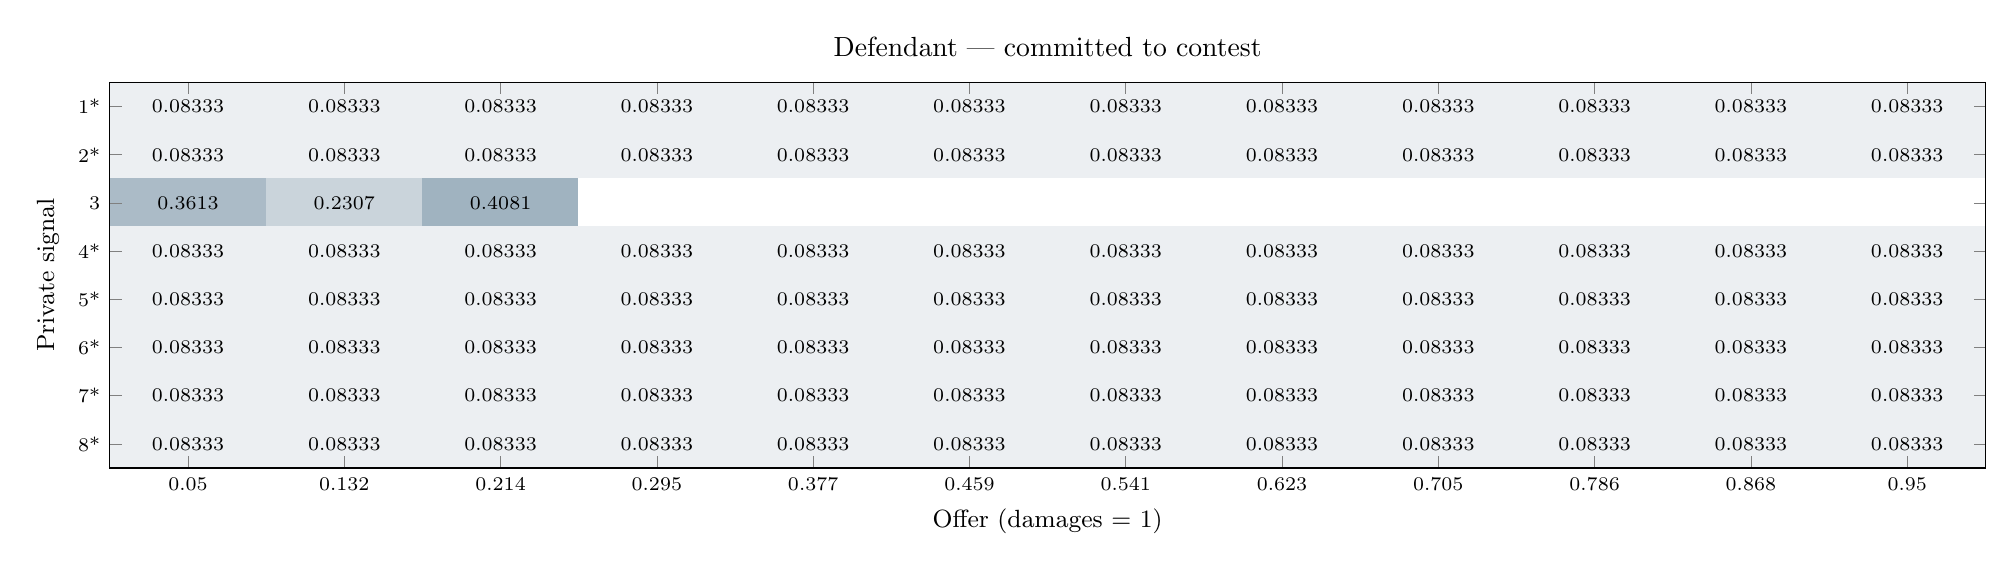
\begin{tikzpicture}\begin{axis}[
width=10.0in,height=2.55in,title={Defendant | committed to contest},
xmin=.5,xmax=12.5,ymin=.5,ymax=8.5,y dir=reverse,
xtick={1,...,12},xticklabels={0.05,0.132,0.214,0.295,0.377,0.459,0.541,0.623,0.705,0.786,0.868,0.95},
ytick={1,...,8},yticklabels={1*,2*,3,4*,5*,6*,7*,8*},
xlabel={Offer (damages = 1)},ylabel={Private signal},
tick label style={font=\scriptsize},label style={font=\small},title style={font=\normalsize},
colormap={policy}{color(0cm)=(white);color(1cm)=(navy)},point meta min=0,point meta max=1,axis on top,clip=false]
\addplot[matrix plot*,mesh/cols=12,point meta=explicit] table[meta=p] {
x y p
1 1 0.083333333333333343
2 1 0.083333333333333343
3 1 0.083333333333333343
4 1 0.083333333333333343
5 1 0.083333333333333343
6 1 0.083333333333333343
7 1 0.083333333333333343
8 1 0.083333333333333343
9 1 0.083333333333333343
10 1 0.083333333333333343
11 1 0.083333333333333343
12 1 0.083333333333333343
1 2 0.083333333333333343
2 2 0.083333333333333343
3 2 0.083333333333333343
4 2 0.083333333333333343
5 2 0.083333333333333343
6 2 0.083333333333333343
7 2 0.083333333333333343
8 2 0.083333333333333343
9 2 0.083333333333333343
10 2 0.083333333333333343
11 2 0.083333333333333343
12 2 0.083333333333333343
1 3 0.36125426691991824
2 3 0.23068241186662022
3 3 0.40806332121346156
4 3 0
5 3 0
6 3 0
7 3 0
8 3 0
9 3 0
10 3 0
11 3 0
12 3 0
1 4 0.083333333333333343
2 4 0.083333333333333343
3 4 0.083333333333333343
4 4 0.083333333333333343
5 4 0.083333333333333343
6 4 0.083333333333333343
7 4 0.083333333333333343
8 4 0.083333333333333343
9 4 0.083333333333333343
10 4 0.083333333333333343
11 4 0.083333333333333343
12 4 0.083333333333333343
1 5 0.083333333333333343
2 5 0.083333333333333343
3 5 0.083333333333333343
4 5 0.083333333333333343
5 5 0.083333333333333343
6 5 0.083333333333333343
7 5 0.083333333333333343
8 5 0.083333333333333343
9 5 0.083333333333333343
10 5 0.083333333333333343
11 5 0.083333333333333343
12 5 0.083333333333333343
1 6 0.083333333333333343
2 6 0.083333333333333343
3 6 0.083333333333333343
4 6 0.083333333333333343
5 6 0.083333333333333343
6 6 0.083333333333333343
7 6 0.083333333333333343
8 6 0.083333333333333343
9 6 0.083333333333333343
10 6 0.083333333333333343
11 6 0.083333333333333343
12 6 0.083333333333333343
1 7 0.083333333333333343
2 7 0.083333333333333343
3 7 0.083333333333333343
4 7 0.083333333333333343
5 7 0.083333333333333343
6 7 0.083333333333333343
7 7 0.083333333333333343
8 7 0.083333333333333343
9 7 0.083333333333333343
10 7 0.083333333333333343
11 7 0.083333333333333343
12 7 0.083333333333333343
1 8 0.083333333333333343
2 8 0.083333333333333343
3 8 0.083333333333333343
4 8 0.083333333333333343
5 8 0.083333333333333343
6 8 0.083333333333333343
7 8 0.083333333333333343
8 8 0.083333333333333343
9 8 0.083333333333333343
10 8 0.083333333333333343
11 8 0.083333333333333343
12 8 0.083333333333333343
};
\node[font=\scriptsize,text=black] at (axis cs:1,1) {0.08333};
\node[font=\scriptsize,text=black] at (axis cs:2,1) {0.08333};
\node[font=\scriptsize,text=black] at (axis cs:3,1) {0.08333};
\node[font=\scriptsize,text=black] at (axis cs:4,1) {0.08333};
\node[font=\scriptsize,text=black] at (axis cs:5,1) {0.08333};
\node[font=\scriptsize,text=black] at (axis cs:6,1) {0.08333};
\node[font=\scriptsize,text=black] at (axis cs:7,1) {0.08333};
\node[font=\scriptsize,text=black] at (axis cs:8,1) {0.08333};
\node[font=\scriptsize,text=black] at (axis cs:9,1) {0.08333};
\node[font=\scriptsize,text=black] at (axis cs:10,1) {0.08333};
\node[font=\scriptsize,text=black] at (axis cs:11,1) {0.08333};
\node[font=\scriptsize,text=black] at (axis cs:12,1) {0.08333};
\node[font=\scriptsize,text=black] at (axis cs:1,2) {0.08333};
\node[font=\scriptsize,text=black] at (axis cs:2,2) {0.08333};
\node[font=\scriptsize,text=black] at (axis cs:3,2) {0.08333};
\node[font=\scriptsize,text=black] at (axis cs:4,2) {0.08333};
\node[font=\scriptsize,text=black] at (axis cs:5,2) {0.08333};
\node[font=\scriptsize,text=black] at (axis cs:6,2) {0.08333};
\node[font=\scriptsize,text=black] at (axis cs:7,2) {0.08333};
\node[font=\scriptsize,text=black] at (axis cs:8,2) {0.08333};
\node[font=\scriptsize,text=black] at (axis cs:9,2) {0.08333};
\node[font=\scriptsize,text=black] at (axis cs:10,2) {0.08333};
\node[font=\scriptsize,text=black] at (axis cs:11,2) {0.08333};
\node[font=\scriptsize,text=black] at (axis cs:12,2) {0.08333};
\node[font=\scriptsize,text=black] at (axis cs:1,3) {0.3613};
\node[font=\scriptsize,text=black] at (axis cs:2,3) {0.2307};
\node[font=\scriptsize,text=black] at (axis cs:3,3) {0.4081};
\node[font=\scriptsize,text=black] at (axis cs:1,4) {0.08333};
\node[font=\scriptsize,text=black] at (axis cs:2,4) {0.08333};
\node[font=\scriptsize,text=black] at (axis cs:3,4) {0.08333};
\node[font=\scriptsize,text=black] at (axis cs:4,4) {0.08333};
\node[font=\scriptsize,text=black] at (axis cs:5,4) {0.08333};
\node[font=\scriptsize,text=black] at (axis cs:6,4) {0.08333};
\node[font=\scriptsize,text=black] at (axis cs:7,4) {0.08333};
\node[font=\scriptsize,text=black] at (axis cs:8,4) {0.08333};
\node[font=\scriptsize,text=black] at (axis cs:9,4) {0.08333};
\node[font=\scriptsize,text=black] at (axis cs:10,4) {0.08333};
\node[font=\scriptsize,text=black] at (axis cs:11,4) {0.08333};
\node[font=\scriptsize,text=black] at (axis cs:12,4) {0.08333};
\node[font=\scriptsize,text=black] at (axis cs:1,5) {0.08333};
\node[font=\scriptsize,text=black] at (axis cs:2,5) {0.08333};
\node[font=\scriptsize,text=black] at (axis cs:3,5) {0.08333};
\node[font=\scriptsize,text=black] at (axis cs:4,5) {0.08333};
\node[font=\scriptsize,text=black] at (axis cs:5,5) {0.08333};
\node[font=\scriptsize,text=black] at (axis cs:6,5) {0.08333};
\node[font=\scriptsize,text=black] at (axis cs:7,5) {0.08333};
\node[font=\scriptsize,text=black] at (axis cs:8,5) {0.08333};
\node[font=\scriptsize,text=black] at (axis cs:9,5) {0.08333};
\node[font=\scriptsize,text=black] at (axis cs:10,5) {0.08333};
\node[font=\scriptsize,text=black] at (axis cs:11,5) {0.08333};
\node[font=\scriptsize,text=black] at (axis cs:12,5) {0.08333};
\node[font=\scriptsize,text=black] at (axis cs:1,6) {0.08333};
\node[font=\scriptsize,text=black] at (axis cs:2,6) {0.08333};
\node[font=\scriptsize,text=black] at (axis cs:3,6) {0.08333};
\node[font=\scriptsize,text=black] at (axis cs:4,6) {0.08333};
\node[font=\scriptsize,text=black] at (axis cs:5,6) {0.08333};
\node[font=\scriptsize,text=black] at (axis cs:6,6) {0.08333};
\node[font=\scriptsize,text=black] at (axis cs:7,6) {0.08333};
\node[font=\scriptsize,text=black] at (axis cs:8,6) {0.08333};
\node[font=\scriptsize,text=black] at (axis cs:9,6) {0.08333};
\node[font=\scriptsize,text=black] at (axis cs:10,6) {0.08333};
\node[font=\scriptsize,text=black] at (axis cs:11,6) {0.08333};
\node[font=\scriptsize,text=black] at (axis cs:12,6) {0.08333};
\node[font=\scriptsize,text=black] at (axis cs:1,7) {0.08333};
\node[font=\scriptsize,text=black] at (axis cs:2,7) {0.08333};
\node[font=\scriptsize,text=black] at (axis cs:3,7) {0.08333};
\node[font=\scriptsize,text=black] at (axis cs:4,7) {0.08333};
\node[font=\scriptsize,text=black] at (axis cs:5,7) {0.08333};
\node[font=\scriptsize,text=black] at (axis cs:6,7) {0.08333};
\node[font=\scriptsize,text=black] at (axis cs:7,7) {0.08333};
\node[font=\scriptsize,text=black] at (axis cs:8,7) {0.08333};
\node[font=\scriptsize,text=black] at (axis cs:9,7) {0.08333};
\node[font=\scriptsize,text=black] at (axis cs:10,7) {0.08333};
\node[font=\scriptsize,text=black] at (axis cs:11,7) {0.08333};
\node[font=\scriptsize,text=black] at (axis cs:12,7) {0.08333};
\node[font=\scriptsize,text=black] at (axis cs:1,8) {0.08333};
\node[font=\scriptsize,text=black] at (axis cs:2,8) {0.08333};
\node[font=\scriptsize,text=black] at (axis cs:3,8) {0.08333};
\node[font=\scriptsize,text=black] at (axis cs:4,8) {0.08333};
\node[font=\scriptsize,text=black] at (axis cs:5,8) {0.08333};
\node[font=\scriptsize,text=black] at (axis cs:6,8) {0.08333};
\node[font=\scriptsize,text=black] at (axis cs:7,8) {0.08333};
\node[font=\scriptsize,text=black] at (axis cs:8,8) {0.08333};
\node[font=\scriptsize,text=black] at (axis cs:9,8) {0.08333};
\node[font=\scriptsize,text=black] at (axis cs:10,8) {0.08333};
\node[font=\scriptsize,text=black] at (axis cs:11,8) {0.08333};
\node[font=\scriptsize,text=black] at (axis cs:12,8) {0.08333};
\end{axis}\end{tikzpicture}
\par\smallskip
{\small Color and cell labels show action probabilities (white = 0; darkest blue = 1). Empty cell labels mean exact zero.
Every positive entry is printed, including arbitrarily small probabilities. Full precision is retained in the editable TeX and profile JSON.}
\end{document}